
\documentclass[a4paper]{resume}

\ResumeName{赖菁}
\usepackage{graphicx}
\usepackage{tikz}
\usepackage{enumitem}

% 防止某些类在双页模式下插入空白页
\makeatletter
\let\cleardoublepage\clearpage
\makeatother

\begin{document}

\ResumeContacts{
  (+86) 188-1158-9056,%
  \ResumeUrl{mailto:3058243931@qq.com}{3058243931@qq.com}
}

\begin{tikzpicture}[remember picture, overlay]
  \node [anchor=north east, inner sep=1cm] at (current page.north east) 
    {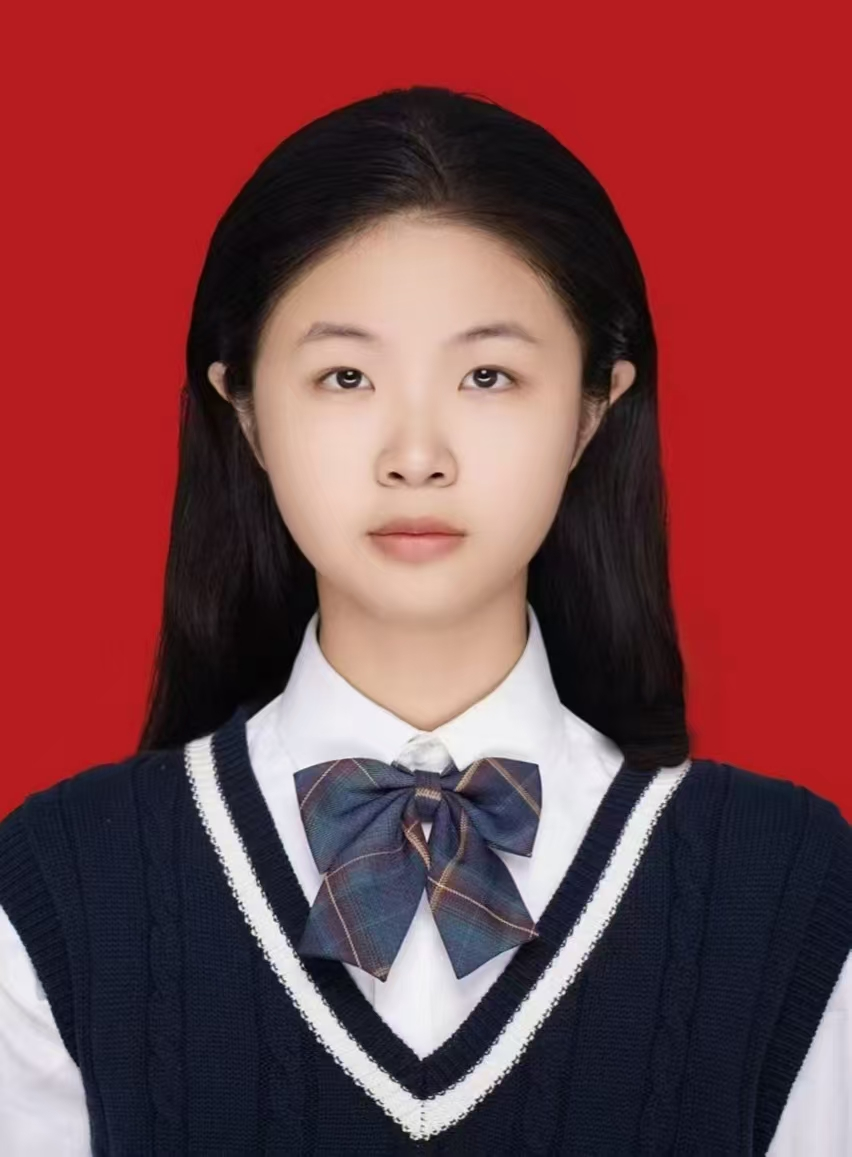
\includegraphics[width=2cm]{head.jpg}};
\end{tikzpicture}

\ResumeTitle

\section{教育经历}
\ResumeItem
[对外经济贸易大学|本科生]
{对外经济贸易大学}
[国际政治\&英语 ， 国际关系学院 | 法学\&文学双学士]
[2024.09—2028.06]
{
  \begin{itemize}[leftmargin=1.5em, itemsep=2pt]
    \item \textbf{学业表现}: 年级排名 \textbf{1/89} | GPA \textbf{3.94/4.00} | 均分 \textbf{91.33}
    \item \textbf{荣誉奖项}: 国家励志奖学金、外研社国才杯"理解当代中国"北京赛区铜奖 (省部级)
  \end{itemize}
}

\section{核心技能}
\begin{itemize}
  \item \textbf{语言能力}: \textbf{英语}可作为核心工作语言，具备出色的双语翻译、外文精读与跨文化交流能力；法语具备基础读写能力。
  \item \textbf{数据分析}: 熟练掌握R语言，能够独立进行数据清洗、爬取与建模分析；具备优秀的结构化分析能力。
  \item \textbf{AI 工具}: 熟悉 AI 行业生态，了解提示词工程。熟练运用AI进行趋势挖掘、文本提炼、内容策划与行业洞察。
  \item \textbf{新媒体设计}: 熟悉公众号运营，熟练掌握Canvas 、秀米等排版工具；熟练使用剪映与 Premiere Pro 进行视频剪辑。
\end{itemize}

\section{实习经历}

\ResumeItem{\textbf{国际青年领袖对话 ( GYLD ) 项目}}
[全球化智库 ( CCG )]
[2026.1 至今]
{
  \begin{itemize}
    \item \textbf{会议统筹与跨部门协作}：深度参与"全球青年领袖年度对话会"及与联合国儿童基金会 ( UNICEF ) 合作的"全球名家对话"等核心品牌活动。负责跨部门沟通与前期物料筹备，独立撰写中英双语会议纪要，保障国际会议落地。
    \item \textbf{媒体矩阵运营}：负责 GYLD 与全球人才组织联合会官方微信公众号、YouTube等多平台的日常运营与数据分析。
    \item \textbf{学术成果宣发}: 跟进 CCG "150 本图书出版成果研讨会"，提升平台内容丰富度与公众影响力。
    \item \textbf{涉外政务翻译}：承担高规格外事活动的文字支持工作，独立完成外宾参访北京通州区的英文推介发言稿翻译，以及通州区代表团出访瑞士、奥地利的官方说明文件英译，保障跨国政企交流的准确性。
  \end{itemize}
}

\ResumeItem{\textbf{国家援外培训项目助理}}
[中华人民共和国商务部]
[2025.11 — 2025.12]
{
  \begin{itemize}
    \item \textbf{双语公文翻译}: 负责"发展中国家参与全球气候治理研修班"的培训手册及会议材料的\textbf{中英互译与校对}，确保外交辞令准确、格式规范
    \item \textbf{涉外事务协调}: 协助主理官员进行外方学员管理，策划并执行跨文化交流活动；负责收集外方需求反馈并建立\textbf{培训数据档案}，保障援外项目高效运转
  \end{itemize}
}

\ResumeItem{\textbf{外文国关传媒实习生}}
[政治学评介]
[2025.09 — 至今]
{
  \begin{itemize}
    \item \textbf{深度选题}: 追踪国际政治领域的热点，协助编辑团队进行选题策划，筛选具有传播价值的外文核心期刊文献
    \item \textbf{学术传播}: 负责将晦涩的英文学术文献编译为通俗易懂的中文推文，锻炼了极强的\textbf{信息提炼能力}与\textbf{文字编辑功底}，确保内容的专业性与可读性并存
    \item \textbf{排版审校}: 负责推文的最终排版与格式校对，严格把控文章的配图质量与排版细节，培养了严谨的内容把控能力
  \end{itemize}
}

\ResumeItem{\textbf{科研助理}}
[对外经济贸易大学 国家安全计算实验室]
[2025.07 — 2025.12]
{
  \begin{itemize}
    \item \textbf{研究主题}:参与金砖国家新能源产业集群合作机制及其发展路径研究，系统梳理俄罗斯、巴西、沙特等\textbf{六国}新能源产业数据。
    \item \textbf{深度分析}:通过比较分析法研究其产业集群特征，协助撰写\textbf{中外产业合作路径分析报告},报告已获\textbf{工信部}认可。
  \end{itemize}
}

\section{校园经历}

\ResumeItem{\textbf{"征途回声"文化传播项目负责人}}
["挑战杯"创新创业大赛红色赛道]
[2024.11 至 2025.04]
{
  \begin{itemize}
    \item \textbf{内容生态建设与商业化策划}：针对文化年轻化传播难点，首创"沉浸式剧本杀 + 红色教育"核心构想。构建"多线剧情架构 + 情感化叙事"的内容生产模型，独立撰写商业计划书并输出标准化实操建议。
  \end{itemize}
}

\ResumeItem{\textbf{校团委项目部干事}}
[对外经济贸易大学 校团委]
[2025.09 — 至今]
{
  \begin{itemize}
    \item \textbf{赛事统筹管理}: 全流程跟进\textbf{"挑战杯"}及科研立项工作，负责数百份申报材料的分类归档与合规性审查
    \item \textbf{数据化运营}: 建立赛事进度数据监控 Excel 表，协调各学院申报进度，确保评审环节零误差推进
  \end{itemize}
}

\ResumeItem{\textbf{院团委宣传部干事}}
[国际关系学院 分团委]
[2024.09 — 2025.06]
{
  \begin{itemize}
    \item \textbf{新媒体矩阵运营}: 独立负责学院官方公众号的内容产出，累计\textbf{独立排版制作推送 24 篇}，涵盖深度报道与活动宣发
    \item \textbf{多媒体制作}: 负责大型活动（迎新晚会、毕业晚会）的摄影采风与后期\textbf{视频剪辑}，提升学院活动的视觉传播效果
  \end{itemize}
}

\end{document}